% Created 2025-10-02 Thu 18:01
% Intended LaTeX compiler: pdflatex
\documentclass[11pt]{article}
\usepackage[utf8]{inputenc}
\usepackage[T1]{fontenc}
\usepackage{graphicx}
\usepackage{longtable}
\usepackage{wrapfig}
\usepackage{rotating}
\usepackage[normalem]{ulem}
\usepackage{amsmath}
\usepackage{amssymb}
\usepackage{capt-of}
\usepackage{hyperref}
\author{Russo Antonio}
\date{2025-09-26}
\title{SRS - Peer-to-Peer Distributed File System}
\hypersetup{
 pdfauthor={Russo Antonio},
 pdftitle={SRS - Peer-to-Peer Distributed File System},
 pdfkeywords={},
 pdfsubject={},
 pdfcreator={Emacs 30.2 (Org mode 9.7.11)}, 
 pdflang={English}}
\begin{document}

\maketitle
\tableofcontents

\section{Introduzione}
\label{sec:org8b1dca9}
\subsection{Scopo}
\label{sec:org3a2e5ad}
Questo documento definisce i requisiti del sistema di File System
Distribuito Peer-to-Peer (P2P FS). Il sistema consente la gestione di file
e directory su più nodi collegati in rete, con accesso trasparente tramite
API remote. Ogni nodo (peer) agisce sia come server che come client.
\subsection{Obiettivi}
\label{sec:orgc3b33ab}
\begin{itemize}
\item Accesso uniforme ai file, sia locali che remoti, tramite RMI.
\item Replica e condivisione dei dati tra peer.
\item Operazioni tipiche di un file system: creazione, lettura, scrittura,
cancellazione, link simbolici e gestione attributi.
\item Robustezza: il fallimento di un peer non blocca l’intera rete.
\end{itemize}
\subsection{Attori}
\label{sec:orgb4e985f}
\begin{itemize}
\item \textbf{Utente}: interagisce tramite il client a riga di comando
\texttt{FileSystemClient}.
\item \textbf{Peer}: nodo che ospita un’istanza di file system distribuito e un
server RMI.
\item \textbf{Rete P2P}: insieme dei peer connessi che replicano ed espongono le API.
\end{itemize}
\section{Descrizione generale}
\label{sec:orgd67b6ab}
\subsection{Architettura}
\label{sec:orgfc6f65a}
Il sistema adotta un modello a \textbf{\textbf{grafo completo}} per rappresentare la rete dei peer.
Ogni nodo mantiene una connessione diretta con tutti gli altri peer della rete.
In questo modo, le operazioni di ricerca e inoltro richieste non richiedono salti multipli,
ma ogni nodo può interrogare direttamente i suoi vicini.
\subsubsection{Vantaggi}
\label{sec:org769eec9}
\begin{itemize}
\item \textbf{Bassa latenza}: le richieste raggiungono il peer interessato in un solo hop.
\item \textbf{Semplicità di implementazione}: non servono algoritmi complessi di routing.
direttamente tra loro senza ricalcolare percorsi alternativi.
\end{itemize}
\subsubsection{Svantaggi}
\label{sec:org5370f4a}
\begin{itemize}
\item \textbf{Scalabilità limitata}: ogni nuovo peer deve stabilire connessioni con tutti gli altri,
portando a un numero di connessioni pari a O(n²).
\item \textbf{Overhead di gestione}: l’aggiunta o rimozione di un peer comporta l’aggiornamento delle
tabelle dei vicini in tutti i nodi.
\item \textbf{Consumo di memoria e risorse}: all’aumentare del numero di peer crescono le risorse
necessarie per mantenere la lista dei vicini.
\end{itemize}
\subsection{Peer}
\label{sec:orgbcbf4e2}
\begin{itemize}
\item Ogni peer possiede un \texttt{FileSystem} montato su una root reale del disco.
\item Il peer espone un server RMI (\texttt{FileSystemServer}) che pubblica un oggetto
remoto (\texttt{RemoteFileSystem}) conforme a \texttt{FileSystemInterface}.
\item I client (\texttt{FileSystemClient}) invocano operazioni sui peer remoti come se
fossero locali.
\end{itemize}
\subsubsection{Inserimento di un nuovo peer}
\label{sec:org245225a}
L’aggiunta di un nuovo nodo avviene tramite la procedura \texttt{joinNetwork}:
\begin{enumerate}
\item Il nuovo peer contatta un nodo bootstrap noto (specificato all’avvio).
\item Il bootstrap fornisce al nuovo nodo la lista dei vicini esistenti.
\item Il nuovo peer stabilisce connessioni con ciascun nodo della lista.
\item In parallelo, ciascun vicino aggiorna la propria tabella aggiungendo il nuovo peer.
\item Durante il join viene effettuato un \textbf{controllo di integrità}: si verifica che non ci
siano conflitti di path già esistenti nei file system dei nodi coinvolti.
\item Se il controllo ha successo, il nodo viene accettato e partecipa a pieno titolo al
grafo completo.
\end{enumerate}
In questo modo, la rete rimane sempre connessa e coerente, garantendo che ogni operazione
possa essere inoltrata a qualsiasi nodo remoto senza ambiguità.
\begin{center}
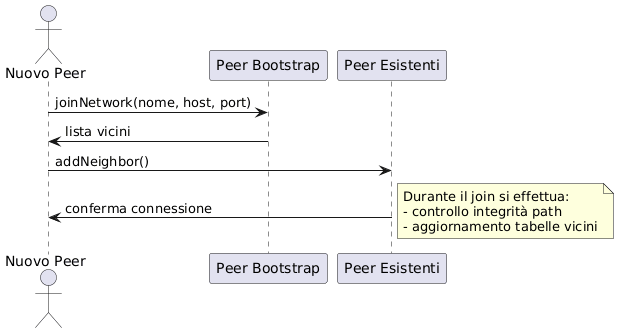
\includegraphics[width=.9\linewidth]{./img/join.png}
\end{center}
\subsection{Vincoli}
\label{sec:org9e06f46}
\begin{itemize}
\item Linguaggio: Java 17+
\item Comunicazione: Java RMI
\item Persistenza: write-through su file system locale
\item Concorrenza: lock tramite \texttt{ReentrantReadWriteLock}
\item Sicurezza: protezione da path traversal
\end{itemize}
\section{Requisiti funzionali}
\label{sec:orgcd3e8ca}
\subsection{Operazioni principali (API esposte)}
\label{sec:org85c4a87}
\subsubsection{Creazione}
\label{sec:orgc82077a}
Le operazioni di creazione seguono il seguente pattern
\begin{enumerate}
\item Il client remoto invia una richiesta remota (es. mknod /path/file\textsubscript{name})
\item Se il path è presente localmente allora il file viene creato utilizzando la primitiva offerta dal file system locale.
\item Se il path non esiste localmente allora la richiesta viene inoltrata ricorsivamente ad un peer remoto.
\item FileSystem acquisisce il lock, aggiorna lo stato in memoria e riflette la modifica su disco locale del peer specificato.
\item Il risultato viene restituito al client.
\end{enumerate}
Questa logica garantisce che ogni operazione possa essere eseguita
in maniera trasparente, sia che il path risieda in locale che in remoto.
\begin{itemize}
\item \texttt{mkdir(path)}: Creazione di una  directory
\end{itemize}
\begin{center}
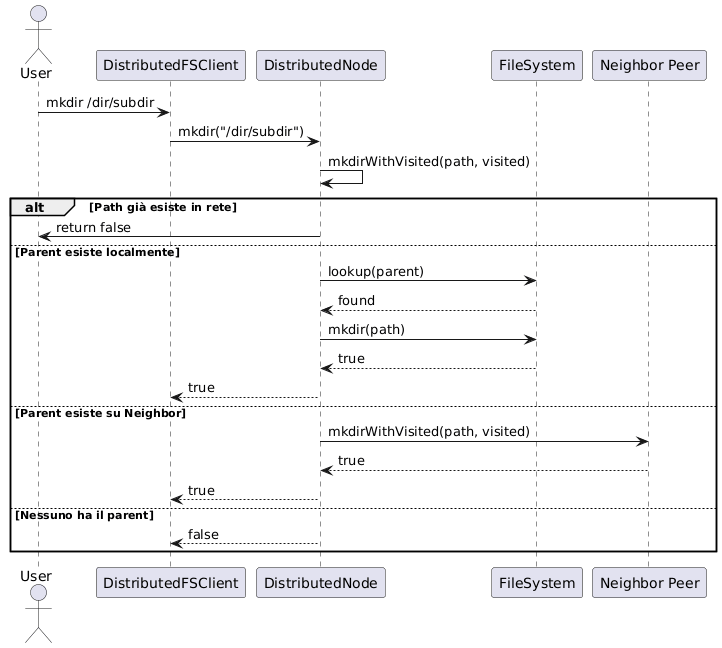
\includegraphics[width=.9\linewidth]{./img/mkdir.png}
\end{center}
\begin{itemize}
\item \texttt{mknod(path)}: Creazione di un  file
\end{itemize}
\begin{center}
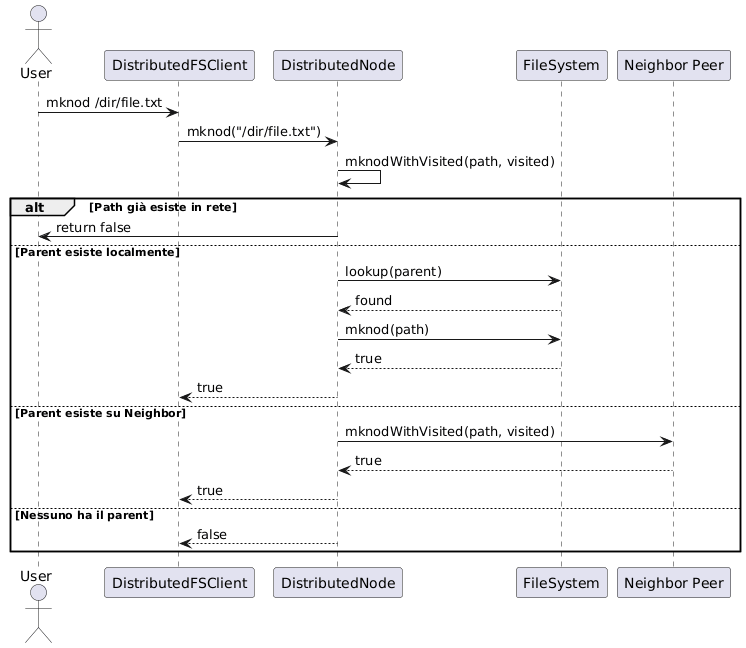
\includegraphics[width=.9\linewidth]{./img/mknod.png}
\end{center}
\begin{enumerate}
\item Consistenza
\label{sec:orge706d97}
la consistenza è garantita grazie ai seguenti passi
\begin{enumerate}
\item Verifica che il nodo da creare (directory, file, symlink) non siano già presenti in locale
\begin{enumerate}
\item Creo il nodo
\end{enumerate}
\item Controllo di integrità \texttt{globale} del path (il nome file non deve essere presente in nessun peer con lo stesso path)
\begin{enumerate}
\item Se il path già esiste allora genero un errore specificando che il file/dir esiste già nel path specificato
\end{enumerate}
\item Se il path (parent) esiste localmente allora gli dò prioorità e lo creo
\item Se il parent esiste in remoto → delego la creazione al peer che lo possiede
\item Se nessuno ha il parent allora l'operazione fallisce con la generazione di un errore
\end{enumerate}
\end{enumerate}
\subsubsection{Manipolazione}
\label{sec:org45c1683}
Le operazioni di manipolazione (scrittura, lettura, rinomina, ecc.) seguono tutte
un flusso generale comune, basato su tre fasi principali:

\begin{enumerate}
\item \textbf{\textbf{Controllo locale}}
Ogni peer controlla prima se il path richiesto è presente nel proprio
\texttt{FileSystem} locale.
\begin{itemize}
\item Se il file o la directory esiste, l’operazione viene eseguita direttamente
in locale, sfruttando i meccanismi di lock e il write-through su disco.
\item Le scritture avvengono in maniera atomica e consistente grazie a
\texttt{ReentrantReadWriteLock}, garantendo che le letture concorrenti
non entrino in conflitto.
\end{itemize}

\item \textbf{\textbf{Inoltro ai vicini (propagazione remota)}}
Se il path non è presente localmente, il peer inoltra la richiesta
ai vicini conosciuti.
Ogni chiamata include una lista \textbf{visited} per evitare cicli infiniti:
se un peer è già stato visitato nella catena della richiesta, la
invocazione viene ignorata.
In questo modo la ricerca termina sempre, anche in presenza di cicli.

\item \textbf{\textbf{Risoluzione e risposta}}
\begin{itemize}
\item Se un peer remoto trova il path, esegue l’operazione e restituisce
il risultato (contenuto letto, conferma di scrittura, lista directory, ecc.).
\item Se nessun peer possiede il path, l’operazione fallisce e viene restituito
un valore di errore.
\end{itemize}
\end{enumerate}
Questa logica garantisce che ogni operazione possa essere eseguita
in maniera trasparente, sia che il path risieda in locale che in remoto.

\begin{itemize}
\item \texttt{write(path, content)}: scrive su file (locale o remoto)
\begin{center}
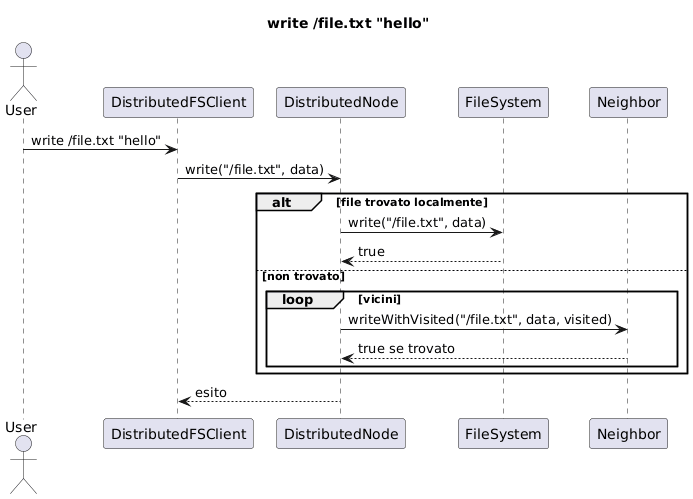
\includegraphics[width=.9\linewidth]{./img/write.png}
\end{center}
\item \texttt{read(path)}: legge contenuto file (locale o remoto)
\begin{center}
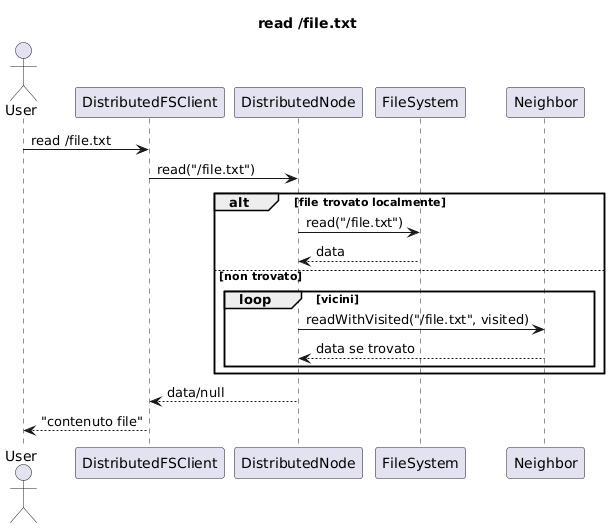
\includegraphics[width=.9\linewidth]{./img/read.png}
\end{center}
\item \texttt{rename(oldPath, newPath)}: rinomina file o directory (locale o remoto).
\begin{center}
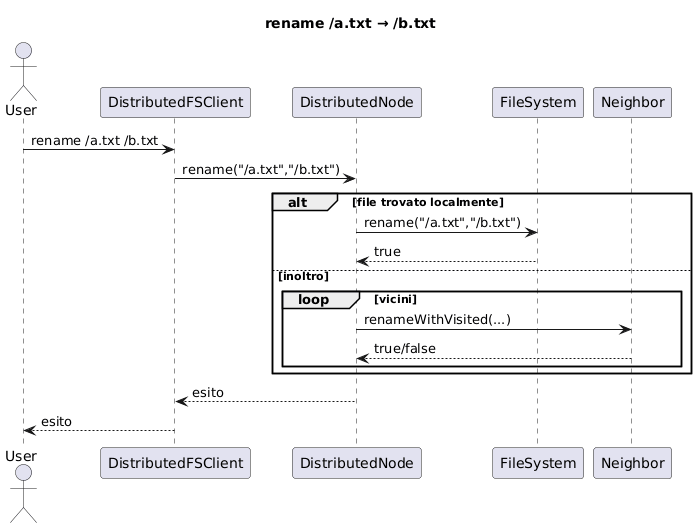
\includegraphics[width=.9\linewidth]{./img/rename.png}
\end{center}
\end{itemize}
\begin{enumerate}
\item Consistenza
\label{sec:orgd8e3334}
La consistenza per le operazioni di manipolazione sono garantite a livello di file system.
\end{enumerate}
\subsubsection{Gestione Attributi}
\label{sec:orgc3bc027}
\begin{itemize}
\item \texttt{readdir(path)}: lista contenuto directory (locale o remoto)
\item \texttt{getattr(path)}: metadati (locale o remoto)
\item \texttt{setattr(path, attr, value)}: modifica attributi
\end{itemize}
\subsection{Funzionalità Client}
\label{sec:org67c0ed6}
\begin{itemize}
\item Interprete comandi interattivo (mkdir, ls, read, write).
\end{itemize}
\section{Requisiti non funzionali}
\label{sec:org4df7e6e}
\begin{itemize}
\item Disponibilità: resilienza alla caduta di nodi.
\item Trasparenza: uniformità tra file locali e remoti.
\item Coerenza: propagazione aggiornamenti ai peer.
\end{itemize}
\end{document}
